\documentclass{article}
\usepackage{graphicx}
\usepackage{subfigure}
\usepackage{natbib}
\usepackage{amsmath}
\usepackage{algorithm}
\usepackage{float}
\usepackage{algorithmic}
\usepackage{hyperref}
\usepackage{IEEEtrantools}
\usepackage{amsmath}
\usepackage{mdframed}
\usepackage{xcolor}
\usepackage{adjustbox}
\usepackage{icml2012}

\newcommand{\theHalgorithm}{\arabic{algorithm}}

\icmltitlerunning{
  Subjective Metadata in Music Classification:
  Genre Prediction via HAC
}

\title{cs4780-fp-report}

\begin{document}

\twocolumn[
\icmltitle{
  CS 4780 Final Project \\
  Subjective Data in Music Classification: \\
  Genre Prediction via Hierarchical Agglomerative Clustering
}
\icmlkeywords{music, nearest neighbors, clustering, danceability}
\vskip 0.3in
]

\begin{abstract}
Music can be numerically quantified in objective terms such as tempo, encoded
chord progressions, lyric term frequencies, and many other features, but how
much can we learn from cold numbers when the appeal of music to humans is in its
subjective attributes? These subjective attributes that model music's impact on
us are difficult to numerically quantify even though they tend to be understood
well by humans. Knowing how much a song might make one want to dance or the
energy of a song helps us better understand what the song might sound like or
the impact it might have on us.
\end{abstract}

\section{Introduction}
Automated music genre prediction has many interesting uses, including the music
recommendation algorithms popular in modern day music applications such as
iTunes' Genius Playlists and Spotify's Suggested Tracks. The majority of the
algorithms that form the basis of these services are privately held and used by
the companies who created them.

We know many of these algorithms use sentimental analysis on the lyrics of songs
for their recommendations, but that comes with its own costs. For one, music
recommendation companies must consider the storage constraints they may encounter
when storing lyrical text for the massive collection of the songs they may recommend.

In that light, we hope to find a less data-intensive way of classifying songs
into genres (the first and most simple step in grouping songs by similarity) by
using song metadata that numerically encapsulates subjective attributes such as
energy and danceability. We hope that in using these subjective attributes, we
will be able to recover some quality of music classification that is lost when
an important portion of the data set is removed: the lyrics.

\section{Problem Definition and Methods}
\subsection{Task Definition}
Our research focuses on the following questions:
\begin{enumerate}
\item Can we re-derive the values of the subjective attributes for a given song
  to better understand the major subjective attributes of the metadata?
\item Can we cluster songs into correct genres using our new understanding of
  the subjective attributes that we obtained from question 1.?
\end{enumerate}

The Echo Nest developers provide no information about how the numerical values
for their subjective attributes were derived, and do not provide a formal
definition for any of the most interesting attributes, which include
\textit{danceability}, \textit{valence}, and \textit{energy}. The only indication
of the meaning of these attributes is in the range of values the attributes can
take, as well as the attribute names.

For example, the attribute \textit{danceability} hints at some measure of how
easy a song is to dance to, but an issue arises in that the ease of dancing is
not well defined. Do we consider a classical song such as Johann Strauss II's
\textit{The Blue Danube}, suitable for graceful waltzes, to be more "danceable"
than the modern hit \textit{Turn Down for What?} by Lil' Jon, which garners
excitement from fist-pumping party-goers?

Exploring the correlations between such subjective attributes allows us to better
predict what significance these attributes might hold. We will provide a
definition of these attributes as we currently understand them in a later section,
but for now, we define what we consider to be the three most important subjective
attributes as we originally defined them:
\begin{itemize}
\item Danceability: How much a song makes a listener want to dance (values in range:
  [0.0..1.0])
\item Energy: Energy from listener point of view (values in range: [0.0..1.0])
\item Valence: Measure of the emotional content of a song (values in range:
  [0.0..1.0])
\end{itemize}

\subsection{Algorithms and Methods}
\subsubsection{Linear Transformation of Data}\label{transform}
We adopted the idea of using a feature mapping to make data linearly separable
in higher dimensions from SVM applications by creating a transformation function
that mapped variables in our data set into a linear shape. In this way, we could
more thoroughly explore the relationship among variables in our data set and how
they relate to our key attributes of danceability, valence, and energy.

To come up with this linear relationship, we used linear fit methods in R to map
our key attributes against the remaining features in the data set. To choose
which variables went into the model, we examined the correlations among variables
in the data. If a variable appeared to be highly correlated with one of the key
attributes, or if it was highly correlated with another variable and contributed
to increasing the linearity of our data, we included it as an interaction term.
In order to measure if the newly added term contributed to making our mapping
more linear, we checked the adjusted $ R^{2} $ value that provides a goodness of
fit test, adjusting for an increase in model parameters, as well as checking the
plotted data to see if the data mapping was visually linear. We stopped adding
terms as soon as the adjusted $ R^{2} $ reached around 70\% in order to prevent
overfitting.

We show our mappings in \textbf{Figures \ref{dance_mapping}, \ref{energy_mapping},}
and \textbf{\ref{valence_mapping}}.

\begin{figure}[H]
  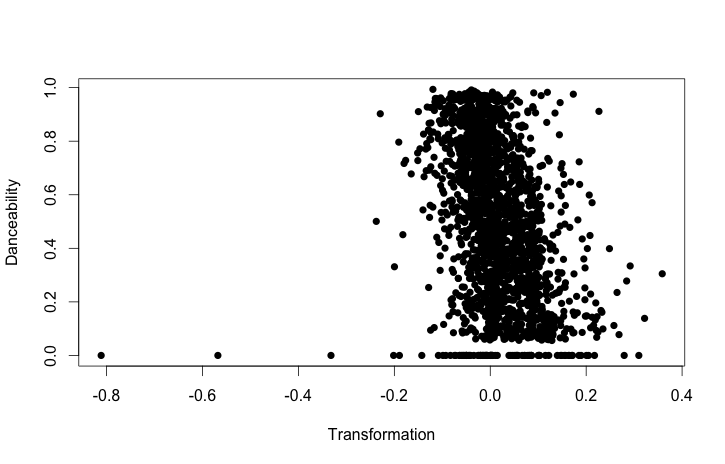
\includegraphics[width=3in]{../images/danceability.png}
  \caption{$ Danceability =
      -3.279225 * 10^{-6} * valence * tempo^{2}
      -8.160651 * 10^{-4} * energy * loudness^{2}
      +3.218223 * 10^{-1} * acousticness * energy^{2}
      -3.279225 * 10^{-6} * liveness * speechiness
      +3.793979 * 10^{-4} * tempo * energy
      -7.492498 * 10^{-3} * loudness * acousticness
      +7.001209 * 10^{-2} * instrumentalness * valence
      -6.132415 * 10^{-4} * valence * loudness
      +1.359087 * 10^{-2} * energy * loudness *valence^{2} $}
  \label{dance_mapping}
\end{figure}

\begin{figure}[H]
  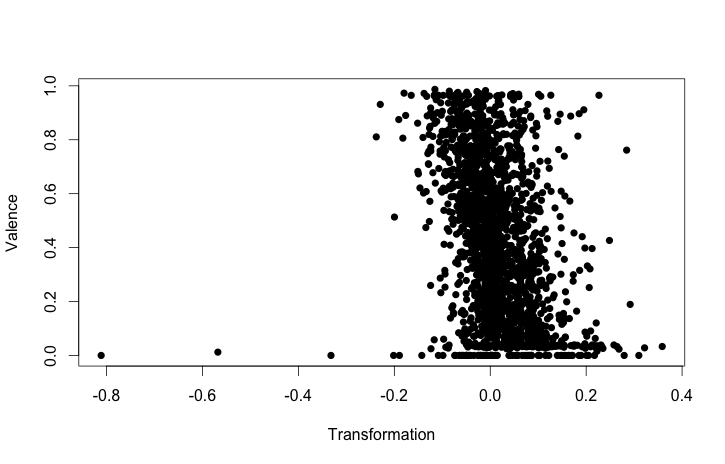
\includegraphics[width=3in]{../images/map_valence.png}
  \caption{$ Valence =
      -3.279225 * 10^{-6} * danceability * tempo^{2}
      -8.160651 * 10^{-4} * energy * loudness^{2}
      +3.218223 * 10^{-1} * acousticness * energy^{2}
      -3.279225 * 10^{-6} * liveness * speechiness
      +3.793979 * 10^{-4} * tempo * energy
      -7.492498 * 10^{-3} * loudness * acousticness
      +7.001209 * 10^{-2} * instrumentalness * danceability
      -6.132415 * 10^{-4} * valence * loudness
      +1.359087 * 10^{-2} * energy * loudness *danceability^{2} $}
  \label{valence_mapping}
\end{figure}

\begin{figure}[H]
  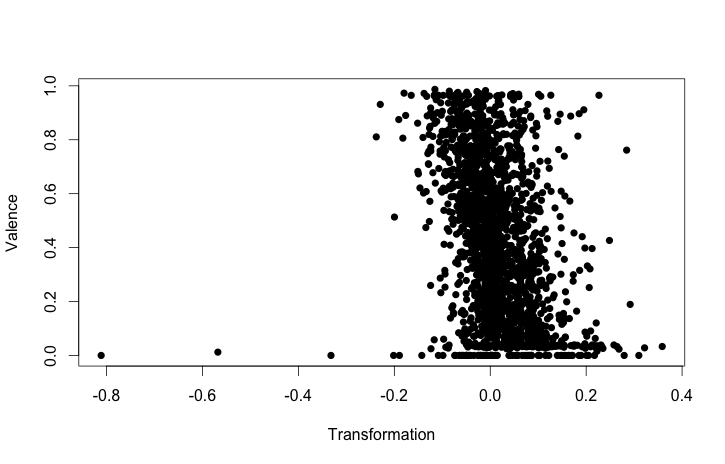
\includegraphics[width=3in]{../images/map_valence.png}
  \caption{$ Energy =
      +3.126570 * 10^{-1} * acousticness
      -7.503000 * 10^{-4} * tempo
      +1.719260 * 10^{-2} * loudness
      -1.399756 * 10^{-1} * valence
      +2.950410 * 10^{-2} * danceability
      -2.433880 * 10^{-1} * speechiness
      +1.868210 * 10^{-2} * loudness * danceability $}
  \label{energy_mapping}
\end{figure}

\subsubsection{k-Nearest Neighbors to Explore the Subjective Metadata}
\textbf{Data Retrieval}\\
We used PHP scripts to pull song data from the Echo Nest API.
We separated that data into two groups:
\begin{enumerate}
\item Training (1800 Songs)
\item Testing (500 Songs)
\end{enumerate}

\textbf{Transformation}\\
With little indication of the exact definition our three primary subjective features
(danceability, energy, and valence), we used the transformations described above
to find the relationship between each of the subjective features to coax out
some sense of how best to define them.

Our more formal definitions of danceability, energy, and valence follow from our
explorations with the transformation:
\begin{itemize}
\item Danceablity: The ease with which a listener can dance to the song, using a
modern dance style. Consistent, upbeat rhythm and high energy.

\item Valence: Low valence corresponds to sadness/ negativity and high valence
corresponds to happiness/ positivity. Corresponds to the x-axis of \textbf{Figure
\ref{energy-valence}}.

\item Energy: How stimulating a song is. Corresponds to the y-axis of \textbf{Figure
\ref{energy-valence}}.

\item Energy and Valence: These two attributes can be combined to form the graph
in \textit{Figure \ref{energy-valence}}, which is used by psychologists describe
emotions. High energy/high valence corresponds to happiness and delightfulness,
while low energy/low valence corresponds to somber moods such as sadness. Low
energy/high valence corresponds to contentedness and calmness, and high energy/
low valence corresponds to strongly negative emotions, such as anger.

\end{itemize}
\begin{figure}[H]
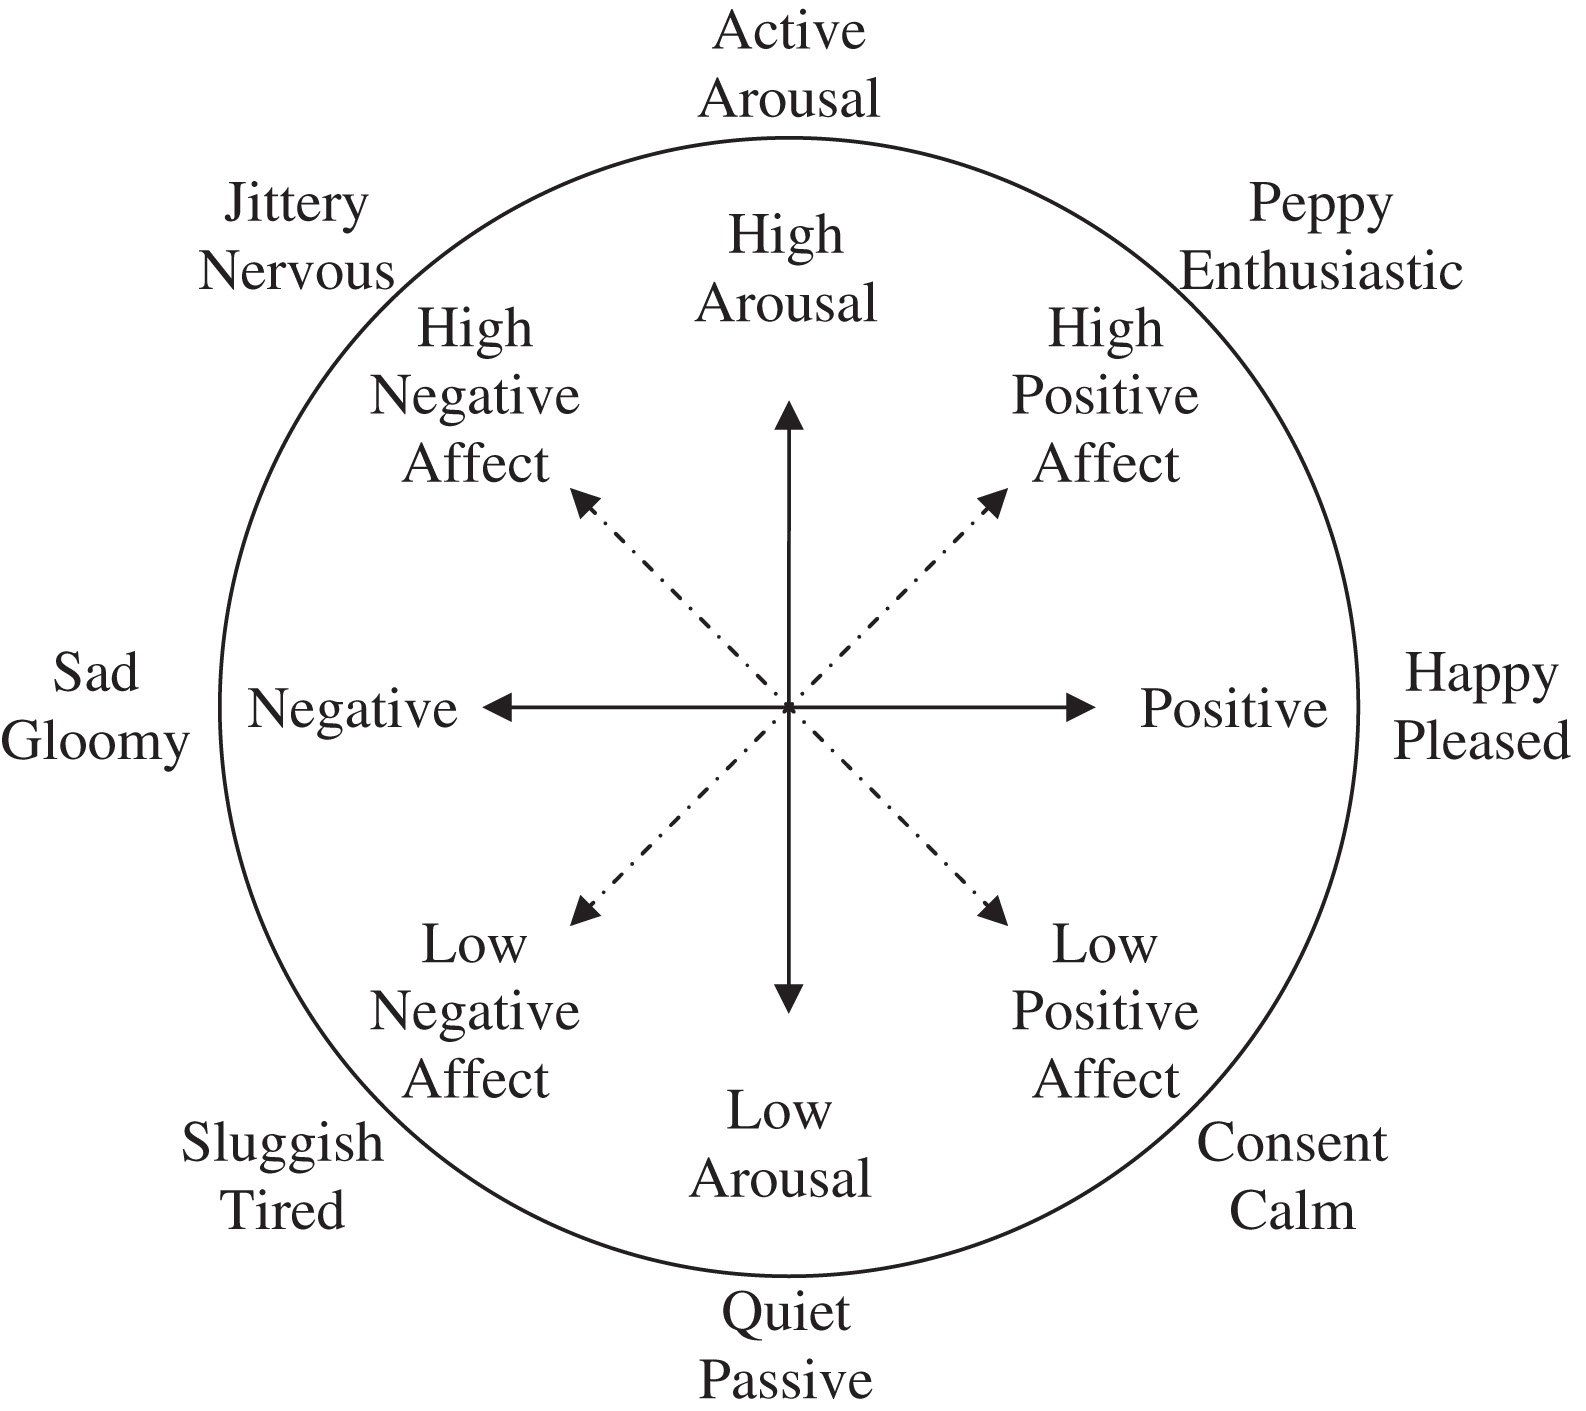
\includegraphics[width=0.5\textwidth]{../images/valence.png}
\caption{
  Mapping of Valence (Negative-Positive) against Energy (High Arousal-Low Arousal)
}
\label{energy-valence}
\end{figure}

\textbf{Similarity Measure}\\
For our baseline tests, we used a Euclidean distance metric on all the numerical
attributes in our data to determine the k-Nearest Neighbors for a given song. We
then compared these results against our results after applying our transformation
to map song data to two dimensions before again using a Euclidean distance metric.
This comparison can be viewed in \textbf{Figures \ref{dance_error}, \ref{energy_error},} and
\textbf{\ref{valence_error}} below.

We used the transformed data to capture the weights of the attributes and their
correlations with other attributes to make sure we maintained the shape of the
data in our attempts to better understand it.

\subsubsection{Hierarchical Agglomerative Clustering for Music Genre Classification}
Our kNN implementation in this research project was used to predict musical
traits of songs based on the probable hypothesis that songs within the same
genre have similar musical properties (danceability, valence, tempo, etc.). To
further correlate the relevance of musical features in our classification, we
used hierarchical agglomerative clustering to study how genres emerge in our
music data set. Specifically, we sought to examine whether the clustering
corresponds to well-defined (as classified by real-world musical experts)
genres, and whether or not songs' nearest neighbors (in the kNN implementation)
are contained within the clustering found via HAC. This would demonstrate the
importance of particular features in the data set, and would indicate if genres
are defined by a range of musical features or whether features are sparse
throughout the feature space.

Our HAC implementation in MATLAB used the single-link (minimum distance),
complete-link (maximum distance), and average-link (average distance) methods to
cluster our song data set. The distance metric we used was Euclidean distance
applied to the song's transformation and valence.

\section{Experimental and Theoretical Evaluation}
\subsection{Data Insight from k-Nearest Neighbors}
\subsubsection{Methodology}
We implemented kNN with and without our transformation function to predict danceability, valence, and energy for a given song and compared the results to check the correctness of our transformation function.

\subsubsection{Results}
The following plots show the runtime and root mean square error based on the number of training samples used with our kNN implementation, both with the transformation and without it:
\begin{figure}[H]
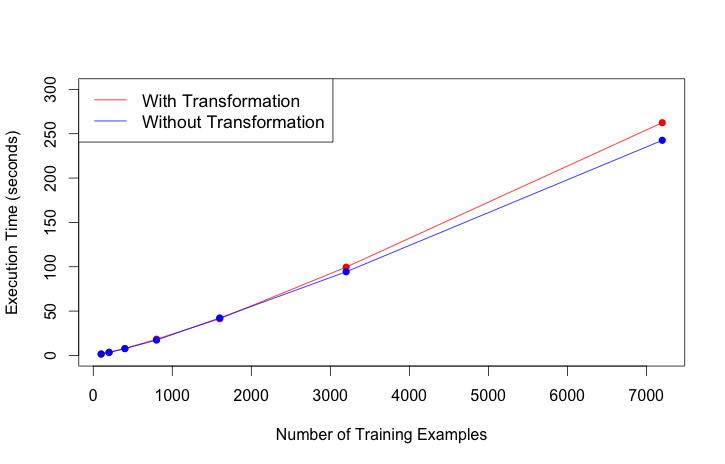
\includegraphics[width=0.5\textwidth]{../images/compare_exec_timeL1.png}
\caption{Comparison of Execution Time}
\label{exec_time}
\end{figure}
\begin{figure}[H]
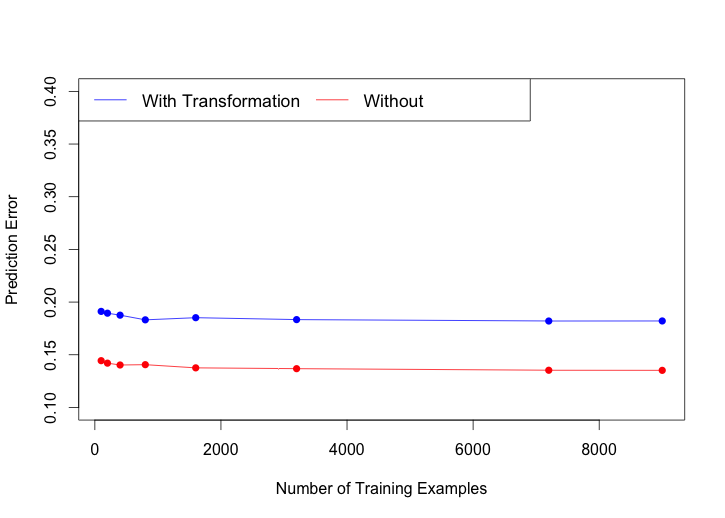
\includegraphics[width=0.5\textwidth]{../images/dance_error.png}
\caption{Comparison of Prediction Error for Danceability}
\label{dance_error}
\end{figure}
\begin{figure}[H]
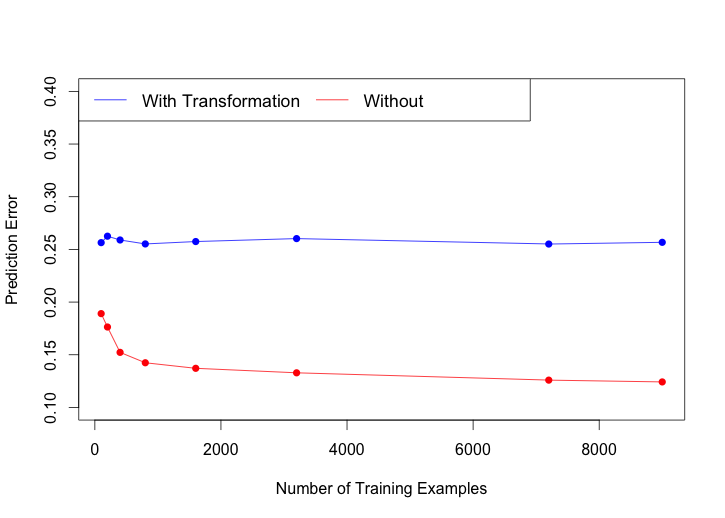
\includegraphics[width=0.5\textwidth]{../images/energy_error.png}
\caption{Comparison of Prediction Error for Energy}
\label{energy_error}
\end{figure}
\begin{figure}[H]
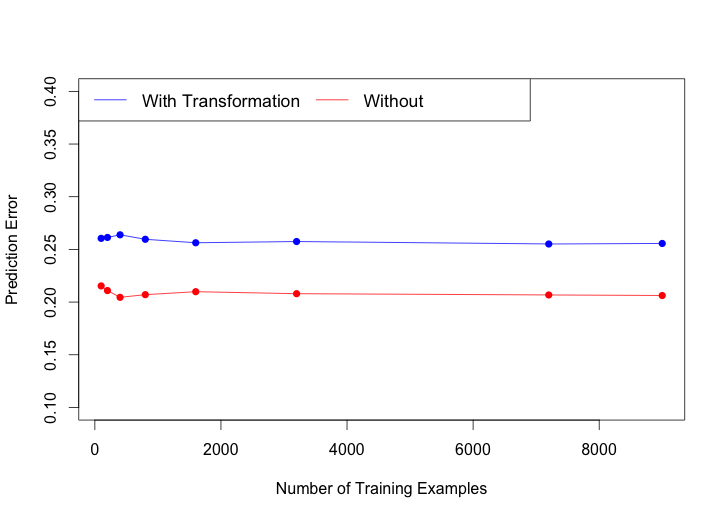
\includegraphics[width=0.5\textwidth]{../images/valence_error.png}
\caption{Comparison of Prediction Error for Valence}
\label{valence_error}
\end{figure}

\subsubsection{Discussion}
Both kNN implementations (with and without the transformation) had similar
execution times, so we can conclude that our transformation does not detract
from the efficiency of kNN.

We also observe that the root mean square error for danceability and valence
only differs about 0.05 units between both implementations of kNN - seeing that
their error rates decrease at essentially the same rate as the number of
training samples increases. Energy on the other hand had a larger difference,
with our transformed data performing at 0.10 worse rate on average, which
reflects on how relatively nonlinear the mapping of energy looked relative to
the danceability and valence maps. So we can assert our transformation function
worked reasonably well with predicting danceability and valence, and could be
improved for predicting energy. We decided to continue using these
transformations that inherently weight the other attributes in our data set for
extensions of our project, including unsupervised genre classification.

\subsection{HAC for Genre Prediction}
\subsubsection{Methodology}
To parallel our work on using kNN to predict unknown features of songs (based on
the hypothesis that similar songs have similar features), we  employed bottom-up
hierarchical agglomerative clustering to learn, without supervision, the genre
structure of the songs in our data set. Using only  the song features provided
by Echo Nest, three methods were used (single link, complete-link, and
average-weighted link) to generate the clustering dendrograms of the data set.

Specifically, our metric was a Euclidean distance algorithm based on the
transformation and two-dimensional instance space from \textbf{Figure
\ref{valence_mapping}}. This transformation was used as it was believed to
capture the interactions between the features in a concise and accurate way.

Using this distance and the three methods listed above, our clustering algorithm
implemented with the MATLAB toolkit output the entire tree-like genre structure
of the song data set. With this dendrogram, our target objective was to
determine how pure and related the genre clusters were; this would be indicative
of whether the features, and their resulting transformation, corresponded well
to genre division, or whether values were not consistently related to genre
structure.

The purity analysis was performed using iTunes and Amazon databases as the genre
supervisors; the genres listed on these databases were used as the true genre
labels in the purity tests.

\subsubsection{Results}
Due to space constraints we could not display all 15 results, but
\textbf{Figures \ref{poor}, \ref{average},} and \textbf{\ref{good}} are
representative samples of the types of clusters we observed.

These figures illustrate the genre clustering towards the root (all-inclusive)
cluster. These clusters were determined via the average-distance metric, and the
percentages indicate the true genre makeup of the learned cluster (and thus
serves as a metric of the accuracy of the cluster).

\begin{figure}[H]
\begin{adjustbox}{minipage=\linewidth-2\fboxrule,bgcolor=gray, frame}
    \centering
	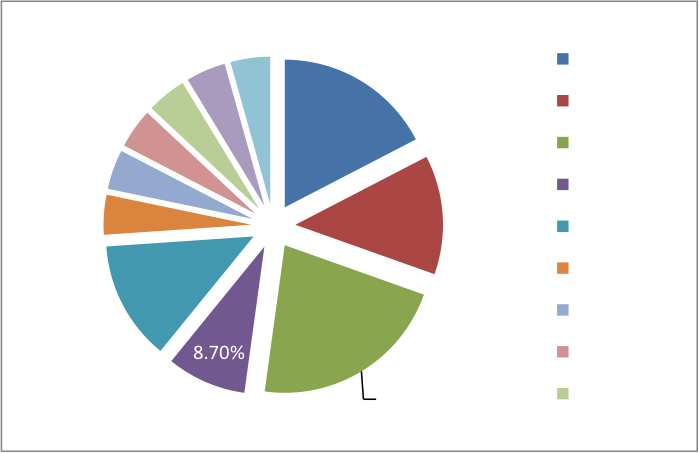
\includegraphics[width=\textwidth, height = 50mm]{../images/c1.png}
\caption{Poor Quality Cluster Example}
\label{poor}
\end{adjustbox}
\end{figure}

\begin{figure}[H]
\begin{adjustbox}{minipage=\linewidth-2\fboxrule,bgcolor=gray, frame}
    \centering
	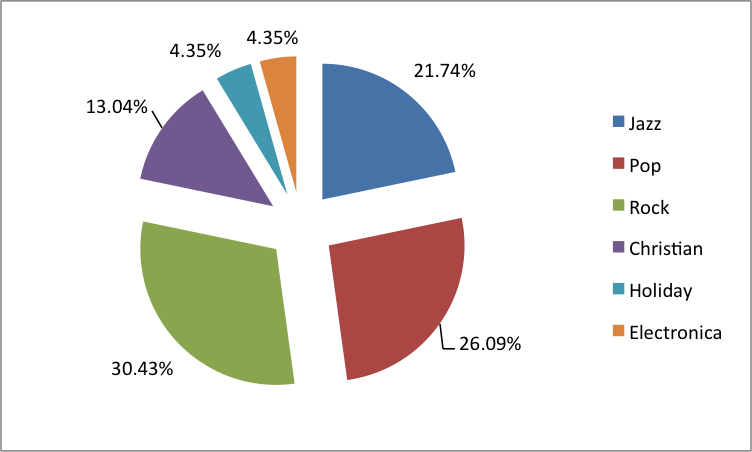
\includegraphics[width=\textwidth, height = 50mm]{../images/c9.png}
\caption{Average Quality Cluster Example}
\label{average}
\end{adjustbox}
\end{figure}

\begin{figure}[H]
\begin{adjustbox}{minipage=\linewidth-2\fboxrule,bgcolor=gray, frame}
    \centering
	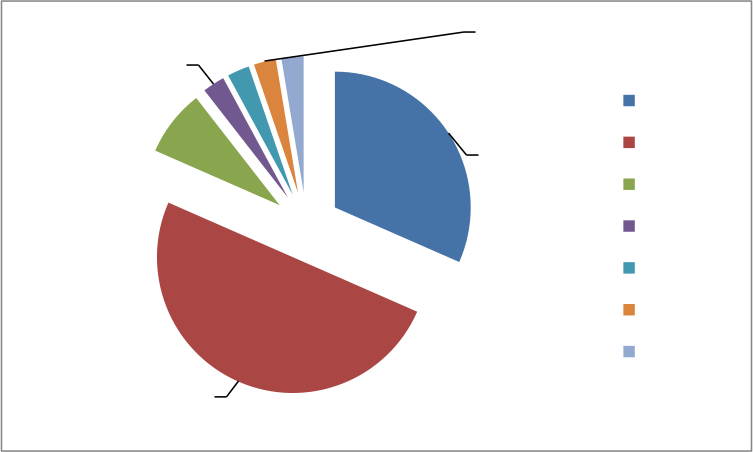
\includegraphics[width=\textwidth, height = 50mm]{../images/c12.png}
\caption{Good Quality Cluster Example}
\label{good}
\end{adjustbox}
\end{figure}

\subsubsection{Discussion}
As demonstrated in the figures, our approach generated clusters of varying
purity. The third cluster is demonstrative of a very well-defined genre (metal
and rock), which leads us to conclude that there is a very strong and
distinctive set of musical features that are found in rock music and metal
music, and that these two genres have many similarities in their attribute features.
On the other hand, the first figure shows a very impure cluster, with several
genres grouped into the same cluster. This is somewhat alarming, as several of
the genres aren't typically associated with each other (i.e. rock and new age).
We can conclude that genres can be defined by similarities of certain music
features weighted by values we found in our transformation function. We were
able to discover several pure or seemingly pure clusters among songs that were
of the same genres if not similar sounding genres. However, we still need to
work to either improve our transformation function or continue finding other
attributes to potentially find purer clusters.

\section{Related Work}
In our research we found a number of similar projects that differ in their focus
on lyrics rather than metadata. Their problem included analyzing lyrics through
the bag of words model and classifying genre solely through the words used. Our
focus on using metadata uses less memory and may be able to classify songs
without having to use natural language processing with some additional work.

\section{Future Work}
Our biggest issue with our data was distinguishing genre between songs that had
similar attribute values. We found that classical songs and rock songs were
often clustered together, and the same with some pop and rock. Something that
could be done to improve this issue would be to include a sentimental analysis,
using a cross section of energy and valence to more accurately represent the
"emotion space." For example, if you have a song that with high danceability and
a romantic feel then it is very likely that it is a pop song, but at the same
time, if the song has a low danceability and a similar romantic feel then it is
more likely to be a rock song. Also, another possible solution would be to
factor in another attribute from the Echo Nest API called Tag. This attribute
has a few keywords that describe and characterize songs. This would also allow
our analysis to make more accurate clusters using a very small amount of string
inputs.

\section{Conclusion}
Thanks to the relatively low error rates from our kNN analysis of attributes, we
were able to understand how danceability, valence, and energy relate to other
attributes in the Echo Nest API. This allowed us to confidently work on an
interesting application of these subjective attributes: genre classification.

From there, we were able to create clusters that were, to some extent, grouped
by similar genres. Although we were not able to generate any pure clusters
composed of only one genre, we still were able to find certain features that
define genres like rock or classical music. These initial results were very
promising and show a bright future for a less data-intensive way to classify
song genres. Hopefully, further work on this subject will cut data and storage
costs for companies and allow for faster and more reliable music sources.

\section{Appendix}
\subsection{Citations and References}
"Echo Nest API Overview." Echo Nest API Overview — The Echo Nest 4.2
Documentation. Web. 9 Dec. 2014. $<$http://developer.echonest.com/docs/v4$>$.

"Hierarchical Clustering Documentation." Hierarchical Clustering. The Math Works
Inc. Web. 9 Dec. 2014.
$<$http://www.mathworks.com/help/stats/hierarchical-clustering-12.html$>$. \\

Joachims, Prof. Thorsten. "Machine Learning Lecture Notes." CS4780 Course, T.
Joachims, Cornell University. Web. 9 Dec. 2014.\\
$<$http://www.cs.cornell.edu/Courses/cs4780/2014fa/$>$. \\

"The Nerve Blog." The Nerve Blog RSS. Web. 9 Dec. 2014.
$<$http://sites.bu.edu/ombs/2011/10/03/gossip-can-influence-perception/$>$.

\subsection{Software}
\begin{itemize}
\item PHP was used for the entirety of the data acquisition and KNN portions of
  our project.
\item HTML, JavaScript, PHP, and CSS were used to create the user interface and
  website that hosted the program. This interface can be viewed using a local
  server such as MAMP, WAMP, or XAMPP and loading \texttt{index.php} in the root
  directory.
\item R was used for the feature mapping of the linear transformation of our
  data attributes.
\item MATLAB was used for the clustering of our data in JSON files.
\end{itemize}

\end{document}
